%%=============================================================================
%% Methodologie
%%=============================================================================

\chapter{Resultaten}
\label{ch:resultaten}

In dit hoofdstuk zullen de resultaten van het experiment besproken worden op basis van de criteria uit sectie \ref{sec:onderzoek}. de verschillende criteria zijn: 
\begin{itemize}
	\item \nameref{sec:moeilijheid}
	\item \nameref{sec:zichtbaarheid}
	\item \nameref{sec:veiligheid}
	\item \nameref{sec:combinatie}
	\item \nameref{sec:voordelen}
\end{itemize}

\section{Moeilijkheidsgraad van de implementatie}
\label{sec:moeilijheid}

Om de moeilijkheidsgraad van de implementatie van een beveiligingsmethode te bepalen kunnen we niet alleen kijken naar de kennis die nodig is om de methode te implementeren maar ook naar alle resources die nodig zijn om een juist implementatie te voltooien. Het aantal resources die nodig zijn voor een beveiligingsmethode kan vaak de doorslag geven of er gekozen wordt voor de ene methode of de andere.

\subsection{Biometric factors}
Als we kijken naar de implementatie met biometrische factoren moet de gebruiker van de applicatie natuurlijk beschikken over de hardware die het uitlezen van deze biometrische factor kan herkennen. Bijna alle nieuwe mobiele toestellen die beschikbaar zijn voor de consument komen met een vingerscanner. Bij het ontwikkelen van de applicatie kan er gemakkelijk gecontroleerd worden of het mobiele toestel beschikt over een vingerscanner of over een andere biometrische factor scanner. Wanneer het mobiele toestel niet beschikt over de nodige hardware om de biometrische factoren te herkennen kan er nog alijd gebruik gemaakt worden van een pincode. Eenmaal geweten dat de authenticatie van de gebruiker zal gebeuren via biometrische scanner of de pincode kan de gebruiken geauthenticeerd worden en krijgt de gebruiker al dan niet toegang te de applicatie en de gegevens. Buiten de pure implementatie van het gebruik van biometrische factoren zal er ook nagedacht moeten worden over de opslag en de beveiliging van de biometrische data die verkregen wordt. 

\subsection{Encryption}
Bij een implementatie met encryptie van de gegevens is er geen nood voor specifieke hardware van het mobiel toestel zoals bij de biometrische factoren. Voor het encrypteren van de gegevens hebben we enkel en encryptie en een decryptie functie nodig om de gegevens te kunnen encrypteren en te decrypteren. Wanneer de gegevens opgevraagd worden door een point-of-sale zullen de gegevens eerst geëncrypteerd worden en dan verzonden worden naar de point-of-sale. Om de werken tussen de applicatie en de point-of-salen goed te laten werken kan er gebruik gemaakt worden van een oplossing van een derde partij die zorgt voor de juiste implementatie aan beide kanten.

\subsection{Tokenization}
Voor tokenization hebben we heel wat meer resources nodig dan bij encryption en biometrische factoren. Om de veiligheid van tokenisatie te garanderen worden de tokens gegenereerd op de server waar de backend op draait. Wanneer de gebruiker een transactie wil doen met de applicatie gebeurt dit aan de hand van een token die werd verkregen via de server en werd gekoppeld aan de gebruiker. Wanneer er een transactie gebeurt via het token zal aan de point-of-sale kant gecontroleerd worden of het token gekoppeld is aan een gebruiker en zo kan de transactie voltooid worden of juist niet als het token niet meer gekoppeld is aan een gebruiker.  

\section{Zichtbaarheid van de gevoelige gegevens}
\label{sec:zichtbaarheid}

\subsection{Biometric factors}
Bij het gebruik van biometrische factoren om uw applicatie te beveiligen kan je enkel toegang krijgen tot de applicatie wanneer uw vingerafdruk gekend is in het systeem of wanneer je de pincode kent wat een groot voordeel is en een groot veiligheidsgevoel geeft aan de gebruiker van de applicatie. Het grote nadeel is dat de gegevens tijdens een transactie als gewone leesbare tekst doorgestuurd wordt. Wanneer eer een aanval gebeurt en de informatie onderschept wordt zijn de gegevens leesbaar voor de aanvaller en kunnen deze misbruikt worden.

\subsection{Encryption}
Wanneer je encryptie implementeert in uw applicatie worden de gevoelige gegeven geëncrypteerd verstuurd. Wanneer de informatie toch onderschept wordt door een aanvaller zijn de gegevens onleesbaar voor de aanvaller. De gegevens kunnen enkel ontcijferd worden wanneer men in bezit is van de sleutel de gebruikt is om de gegevens te encrypteren. De gegevens zijn dus zichtbaar bij de invoer ervan of wanneer ze gedecrypteerd worden.

\subsection{Tokenization}
Bij tokenisatie worden de gevoelige gegevens vervangen door random gegenereerd token die niet ontcijfert kan worden. Dit token wordt gebruikt in plaats van de gevoelige gegevens en wordt dus doorgestuurd wanneer een transactie gedaan wordt. Aangezien alles via een token verloopt zijn de gegevens enkels zichtbaar bij de ingave, het verschil met encryptie is dat het token niet ontcijferd kan worden.

\section{Veiligheid van de beveiligingsmethode}
\label{sec:veiligheid}

\subsection{Biometric factors}
Biometrische factoren zoals gezichtsherkenning, irirsscan, spraakherkenning en vingerscan praktisch niet na te bootsen, vingerscan kan omzeild worden als de aanvaller de vingerafdruk van de gebruiken kan bemachtigen. Wanneer men werkt met biometrische factoren is er altijd een back-up met een pincode. Een pincode kan gemakkelijk gekraakt worden via brute force aanvallen (dit is een aanval die alle mogelijke combinaties probeert tot de juiste combinatie gevonden is). Er kan natuurlijk een extra regel voorzien worden dat er maar een bepaald aantal pogingen gedaan mogen worden om de applicatie te ontgrendelen. Zolang de aanvaller niet voorbij deze beveiligingen raakt heeft hij geen toegang tot de gegevens van de gebruiker.
 
\subsection{Encryption}
Geëncrypteerde data kan enkel ontcijfert worden als men in bezit is van de sleutel waarmee de data is geëncrypteerd. Een aanvaller kan proberen om de data te ontcijferen zonder de encryptie sleutel door middel van een brute force aanval. Net zoals bij een brute force aanval voor een pincode zal hier alle mogelijke combinaties geprobeerd worden tot dat de sleutel gevonden is. Hoe langer of groter de sleutel is hoe langer het duurt vooraleer een brutef orce aanval de sleutel kan ontcijferen. In figuur \ref{fig:bruteForce} ziet u een representatie van hoe lang het duurt om een geëncrypteerd wachtwoord te ontcijferen invergelijking met het aantal karakters van het wachtwoord ~\autocite{BruteForce}.

 \begin{figure}
	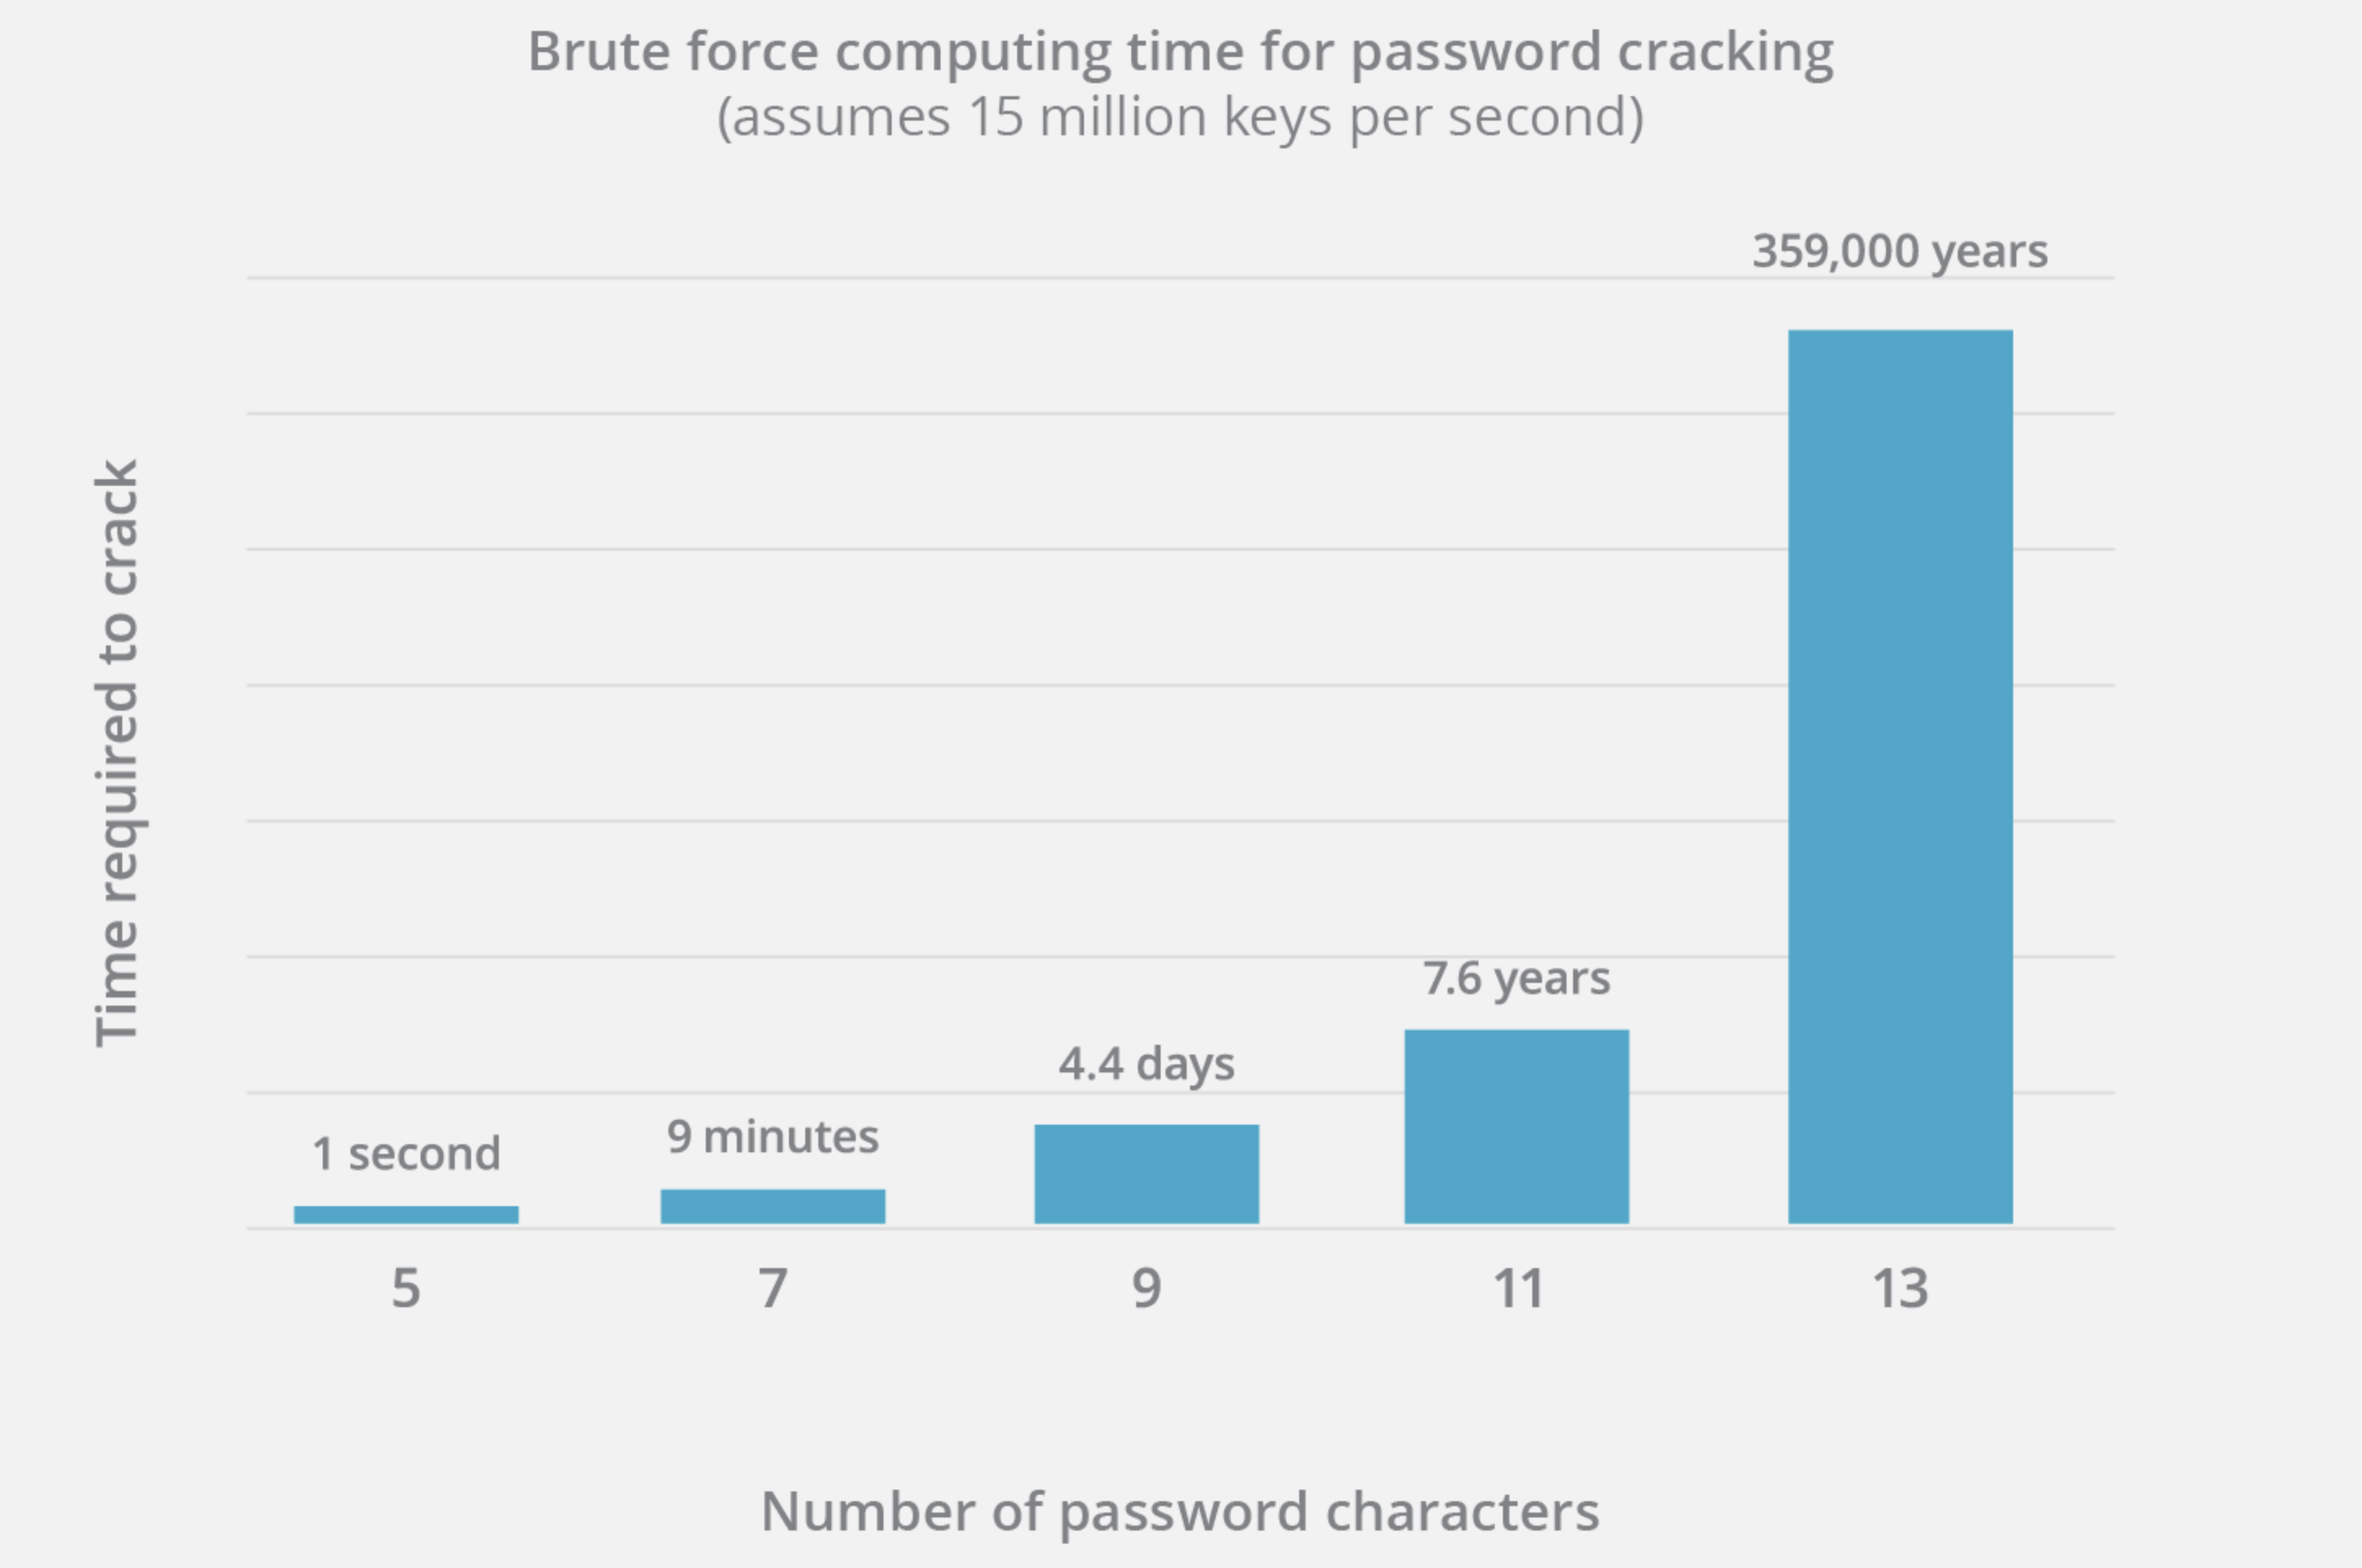
\includegraphics[width=\linewidth]
	{img/bruteforce}
	\caption{Representatie van de nodige tijd om een geëncrypteerd wachtwoord te ontcijferen}
	\label{fig:bruteForce}
\end{figure}

\subsection{Tokenization}
Bij tokenisatie wordt er gebruikgemaakt van tokens, dit is een reeks van tekens die willekeurige gegenereerd worden. Aangezien de tokens willekeurig gegenereerd worden en geen gegevens bevatten kunnen ze dus ook niet ontcijfert worden. Wanneer er gebruikt gemaakt wordt van eenmalige tokens kan de aanvaller hier niets mee aanvangen eenmaal ze onderschept zijn. Als het gaat om tokens die meermaals gebruikt kunnen worden kan de aanvaller zich voordoen als de rechtmatige gebruiker van de tokens. De aanvaller kan gebruikmaken van de tokens tot de levensduur van de tokens vervallen zijn of tot wanneer ze uit het systeem verwijdert zijn door het opmerken en het melden van de aanval.

\section{Combinatie van verschillende beveiligingsmethodes}
\label{sec:combinatie}
Het is mogelijk om de verschillende beveiligingsmethodes te combineren met elkaar. Er kan gekozen worden om een applicatie met encryptie te combineren met biometrische factoren of tokenisatie te combineren met biometrische factoren. Zo is de toegang tot de betalingsapplicatie beveiligd en worden de gegevens beveiligd verstuurd. Encryptie en tokenisatie kunnen ook perfect gecombineerd worden hierbij worden de gegevens eerst geëncrypteerd en dan verzonden naar de server om daarvoor dan een token te laten genereren. Het is ook mogelijk om alle drie van de gekozen beveiligingsmethodes te combineren met elkaar. Dit zorgt voor beveiligde toegang tot de applicatie, data die geëncrypteerd verstuurd wordt naar de server om dan een niet ontcijferbare token te genereren waarmee transacties geautoriseerd kunnen worden. Dit onderzoek beperkt zich nu tot deze drie methodes maar het is ook mogelijk om andere methodes uit sectie~\ref{sec:Beveiliging} te cojbineren met elkaar.

\section{Voordelen van het combineren van verschillende methodes}
\label{sec:voordelen}
Het combineren van verschillende beveiligingsmethodes zorgt logischerwijs voor extra voordelen namelijk extra veiligheid. Wanneer we enkel een implementatie doen van biometrische factoren is enkel de toegang tot de applicatie beveiligd maar niet het versturen van de gevoelige gegevens. Bij de implementaties met encryptie en tokenisatie is het versturen van de gevoelige gegevens van de gebruiker wel beveiligd maar de toegang tot de applicatie is vrij. Wanneer we biometrische factoren combineren met encryptie ofwel tokenisatie zorgt dit voor een extra beveiligingslaag namelijk de toegang tot de applicatie zelf. Zoals in het in sectie \ref{sec:combinatie} al vermeld werd kunnen ook alle drie van deze beveiligingsmethodes gecombineerd worden met elkaar en zorgt dit weer voor een extra beveiligingslaag voor de applicatie. Er moet ook wel rekening mee gehouden worden wanneer men kiest voor een combinatie van verschillende beveiligingsmethodes of dit wel nodig is voor de specifieke use-case, als het gaat om een simpele loyalty applicatie (bijvoorbeeld klantenkaart om punten te sparen) dan is een combinatie van tokenisatie en biometrische factoren misschien overbodig door de hogere kost die erbij komt bij het implementeren van tokenisatie. Het combineren van biometrische factoren met encryptie of tokenisatie kan ook op een andere manier bekeken worden dan puur op de extra veiligheid van de applicatie, het implementeren van biometrische factoren in een applicatie zorgt voor een groter veiligheidsgevoel bij de gebruiker. Dit zorgt voor een grotere user-experience wat op zicht zorgt voor een grotere klanten tevredenheid.